%Chapter 6
\chapter{Theoretical Background: LDPC Construction} \label{ldpc_chap}
\label{chapter6}
This chapter gives some minimal amount of background to understand and examine Error Correcting Codes in general, 
definitions of basic terms, LDPC code construction and their properties\cite{shaishav_mtp}.


\section{LDPC Construction} 

Consider an LDPC code \cite{ecc_shu_lin} $C$ of length $n$ specified by $n\times n$ parity-check matrix $H$.
Now onward we will focus on regular, cyclic LDPC codes, with number of rows $J=n$
and $\rho=\gamma$.

Let $h_{1}, h_{2},.., h_{n}$ denotes rows of H where
\begin{center}
 $\mathbf{h_{j}}=(h_{j,0},h_{j,1},\cdot \cdot \cdot,h_{j,n-1} ) $
\end{center}

For $1\leq j \leq n$, let $u= (u_{0}, u_{1},\cdot \cdot \cdot,u_{n-1})$ be a code word in C,
then the inner product,
\begin{align*}
  \mathbf{v_{j}=u \cdot h_{j}}=\sum_{l=0}^{n-1}u_{l} h_{j,l}=0 
\end{align*}


gives the parity check sum (parity-check equation).

The parity-check sums in $v_{l}$ are said to be orthogonal on bit node $u_{l}$.
For every bit node of regular LDPC code$C$, there are $\gamma$ parity-check sums
that are orthogonal on it. Using this LDPC code, any error pattern with $\leq \gamma /2$
error can be corrected.
Hence the minimum distance $d_{min} \geq \gamma +1$.

LDPC codes can be constructed using two families of finite geometry:
\begin{enumerate}
 \item Projective Geometry (PG)-LDPC Codes
 \item Euclidean Geometry (EG)-LDPC Codes
\end{enumerate}

The system which we are implementing is derived completely from \textbf{\textit{PG-LDPC}}
construction. Hence we will focus only on PG-LDPC codes.

\subsection{Parameters of PG LDPC Code}
Two-dimensional PG-LDPC codes have following parameters\cite{ecc_shu_lin}:
\begin{itemize} \label {ldpc_parameters}
\NumTabs{6}
 \item Length \tab{} \tab{$n=2^{2s}+2^{s}+1$}
 \item Number of parity bits \tab{$n-k=3^{s}+1$}
 \item Dimension \tab{} \tab{$k=2^{2s}+2^{s}-3^{s}$}
 \item Minimum Distance \tab{$d_{min}=2^{s}+2$}
 \item Density \tab{} \tab{$r=\frac{2^{s}}{2^{2s}+2^{s}+1}$}
\end{itemize}
The parity-check matrix $\mathbf{H_{PG}}$ of PG-LDPC code is a $(2^{2s}+2^{s}+1)\times (2^{2s}+2^{s}+1)$
square matrix. \cite{ecc_shu_lin}, which can be obtained by taking the incidence vector of a line 
in $\mathbf{H_{PG}}$ and its $2^{2s}+2^{s}$ cyclic shifts as rows.

By substituting different values of parameter $s$ in List-\ref{ldpc_parameters}, we can obtain the 
Table-\ref {ldpc_parameter_table}   
 
 \begin{table} [!h]
 \caption{Two-Dimensional PG-LDPC code Parameters}
  \begin{center}
 \begin{tabular}{||c c c c c c c||} 
 \hline
  &Length &Dimension & Minimum Distance & Row Weight & Column Weight & Density\\ %[0.5ex] 
 $s$ & $(n)$ & $(k)$& $(d_{min})$ & $(\rho)$ & $(\gamma)$ & $(r)$ \\ %[0.5ex] 
 \hline
 1 & 7 & 3 & 4 & 3 & 3 & 0.4286\\ 
 2 & 21 & 11 & 6 & 5 & 5 & 0.2381\\ 
 3 & 73 & 45 & 10 & 9 & 9 & 0.1233\\ 
 4 & 273 & 191 & 18 & 17 & 17 & 0.0623\\
 5 & 1057 & 813 & 34 & 33 & 33 & 0.0312\\
 6 & 4161 & 3431 & 66 & 65 & 65 & 0.0156\\
 7 & 16513 & 14325 & 130 & 129 & 129 & 0.0078\\
   \hline
\end{tabular}
\end{center}
\label{ldpc_parameter_table}

\end{table}

Decoder is implemented for the following structure.
$\mathbf{PG-LDPC\ (7,3)}$ with $\mathbf{s=1}$

In the upcoming chapters, we will focus mainly on this architecture for partitioned and un-partitioned NoC implementation. The concept can be applied to any of the LDPC. Hence the conclusion will be general.  

\subsection{Parity-check Matrix}
The LDPC code which we are going to implement is a linear block code, regular and cyclic code.
The parity-check matrix for $PG-LDPC\ (7,3)$ is given below.

\begin {equation} \label{h_7x7}
H=
\begin{bmatrix} 
0 & 0 & 0 & 1 & 0 & 1 & 1 \\
1 & 0 & 0 & 0 & 1 & 0 & 1 \\
1 & 1 & 0 & 0 & 0 & 1 & 0 \\
0 & 1 & 1 & 0 & 0 & 0 & 1 \\
1 & 0 & 1 & 1 & 0 & 0 & 0 \\
0 & 1 & 0 & 1 & 1 & 0 & 0 \\
0 & 0 & 1 & 0 & 1 & 1 & 0 \\ 
\end{bmatrix}
\end {equation}

This matrix is obtained by keeping $d_{min}=4$, define a tuple $u= (0,0,0,1,0,1,1)$ and 
apply shifting operation $6\ times$ for each row.
The Tanner graph constructed from the parity check matrix of Equation- \ref{h_7x7} is given in 
Figure- \ref{tanner_graph_for_parity_check}.
$u_{i}$ represents the $i^{th}$ row. $v_{j}$ represents the $j^{th}$ column.
An edge between $u_{i}$ and $v_{j}$ exist if $H [i][j]=1$ in the parity check matrix specified in Equation-\ref{h_7x7}.


\begin{figure}[H]
  \centering
   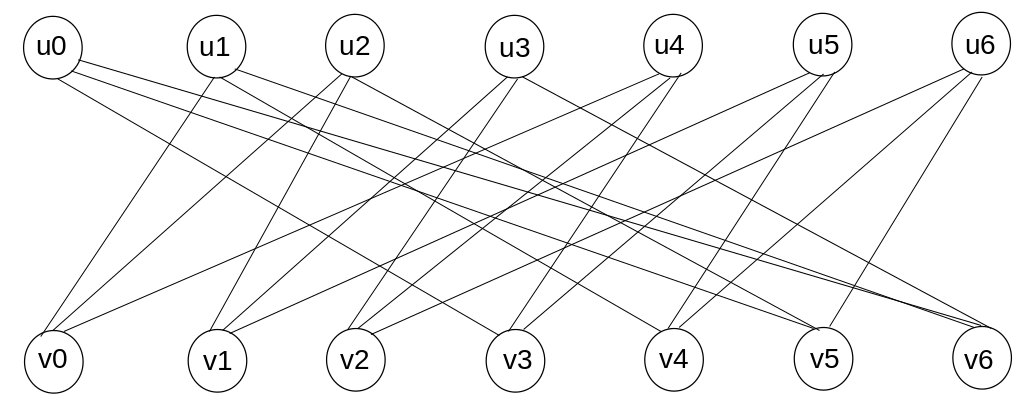
\includegraphics[scale=0.3]{./figs/tanner_graph_for_parity_check}
  \caption{Tanner Graph representation for Parity Check Matrix of equation \ref{h_7x7}}
  \label{tanner_graph_for_parity_check}
\end{figure}


 In LDPC Decoder implementation, \textbf{\textit{5 bit precision}} for all the bit nodes and check node message is used.
 Out of which, \textbf{\textit{1 bit for sign}}, \textbf{\textit{3 bit of integer}} and \textbf{\textit{1 bit of fraction precision}} should be 
 considered. 
 
 
\begin{figure}[H]
  \centering
   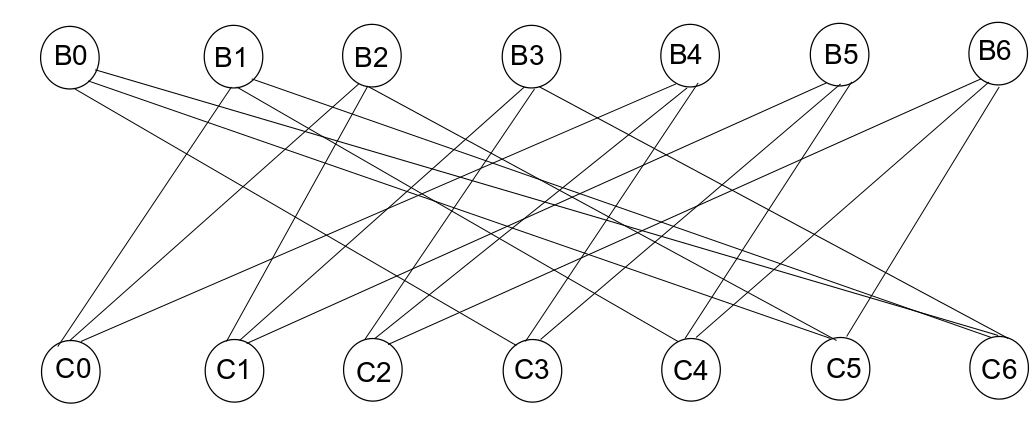
\includegraphics[scale=0.4]{./figs/tanner_graph}
  \caption{Tanner Graph representation of (7,3) Block-code}
  \label{tanner_graph}
\end{figure}

 Figure- \ref{tanner_graph} shows the Tanner graph representation of (7,3) Block code. This code is implemented in next chapter.
 PG-LDPC (73,45) code is implemented as $Linear\ Block\ code\ (73,45)$, where $73$ represents length of code and $45$ is the dimension.\\